% ============================================================
% 分片：s03c  对应原文 PDF 第 41--44 页
% 负责章节：§3.2 Homotopy-algebraic considerations；§3.2.1 Topological quantum mechanics and $A_\infty$ algebras
% 译者：translator-06   审校状态：初稿
% ============================================================

% ==== 原文 PDF 第 41 页 ====
\subsection{同伦代数方面的考量}

已经可以看到，扭变超对称量子场论中的代数结构可以极为丰富。事实上，链层面的代数结构还可以更丰富，这符合预期，因为 $Q$-恰当项此时尚未被丢弃。这一语境所需的相关代数结构有时称为高阶代数（higher algebras）或同伦代数（homotopy algebras）。它们在数学与物理中都是深刻而往往令人生畏的结构，因此我们将把大部分篇幅用于讨论其中最著名的例子：$A_\infty$ 代数。粗略地说，$A_\infty$ 代数就是同伦意义下的结合代数；类似地，$L_\infty$ 代数只满足同伦意义下的 Lie 代数公理，下文将会看到。这些额外结构可以以精巧的方式在对偶之间转移。

\subsubsection{拓扑量子力学与 $A_\infty$ 代数}

下面从最简单的情形开始：一个扭变的量子力学（一维）理论。3.1 节通过考察 $\mathbb{R}$ 中两点的构型空间看到，局域算子的 $Q$-上同调是一个未必交换的代数。也看到，考察三点的构型空间意味着局域算子（的 $Q$-上同调类）的碰撞乘积还是结合的。特别地，给定三个 $Q$-闭局域算子 $O_1$、$O_2$ 与 $O_3$，可得结合子（associator）$(O_1O_2)O_3 - O_1(O_2O_3)$ 在 $Q$-上同调中是平凡的；下面研究这一结合子是如何被平凡化的。

首先，用 $\mathbb{R}$ 上两个（不同）点（更确切地说，开区间）的构型空间同调来重述二元碰撞。该构型空间有两个连通分支，分别对应 $x_1<x_2$ 与 $x_1>x_2$；我们聚焦于 $x_1>x_2$ 的分支，它可与一个半空间等同。总可以利用整体平移取 $x_1=-x_2$，于是选定整体标度（即 $x_1-x_2$ 的值）之后，约化构型空间就是单点 $\mathcal{K}_2$。次数为 0 的乘积 $O_1O_2$ 来自该约化构型空间上一个积分的 $x_1-x_2\to0$ 极限：
% [Tutor Note: 物理图像：$\mathcal{K}_2$ 是把两点构型用平移与整体缩放约化后剩下的“形状空间”，故碰撞乘积本质上是该空间基本类上的积分；(3.10) 中的 $\star_\Gamma$ 是这一构造的链层面推广。]
\begin{equation}\tag{3.17}
O_1O_2 = \lim_{x_1-x_2\to0}\int_{\mathcal{K}_2}(O_1(x_1)O_2(x_2))^{(0)} = \lim_{x_1-x_2\to0}\int_{\mathcal{K}_2}O_1(x_1)O_2(x_2).
\end{equation}

更确切地说，应选取一个用于点分裂（point-splitting）的小正参数 $\epsilon$，改为取 $x_1-x_2\to\epsilon$；（正规化后的）乘积 $O_1O_2$ 由去掉对 $\epsilon$ 奇异的项、再取 $\epsilon\to0$ 极限得到。这就是上述 $x_1-x_2\to0$ 极限的含义。关于局域算子的点分裂，细节参见 [75, Chapter 2]。特别地，最好把局域算子看作小的开区间而非单纯的点。无论哪种看法，超荷 $Q$ 都是该乘积的费米子导子：
% [Tutor Note: 易错预警：这里的 $x_1-x_2\to0$ 是记号而非字面极限；实际取的是“减去 $1/\epsilon$ 等奇异项之后”的极限，故写 $O_1O_2$ 时已隐含正规序。计算中若出现 $\epsilon$ 极点，须先减除再取极限。]
\begin{equation}\tag{3.18}
Q(O_1O_2) = (QO_1)O_2 + (-1)^{F(O_1)}O_1(QO_2).
\end{equation}

同样的分析适用于 $x_1<x_2$ 的分支，那里得到相反次序的（0 次）乘积 $-(-1)^{F(O_1)F(O_2)}O_2O_1$（对算子的宇称取合适的符号）。$\mathbb{R}$ 上三个点（或开区间）的构型空间有六个连通分支，对应 $6=3!$ 种可能的次序。把构型平移到 $x_1=-x_3$ 并选取
% ==== 原文 PDF 第 42 页 ====
整体标度 $x_1-x_3$ 后，得到满足 $x_1>x_2>x_3$ 的约化构型空间，它就是一个区间
\begin{equation}\tag{3.19}
\mathcal{K}_3(\epsilon) = \{x_2\in\mathbb{R} \mid x_3+\epsilon \le x_2 \le x_1-\epsilon\}.
\end{equation}

这里显式地引入点分裂参数 $\epsilon$，并要求 $x_1-x_3\ge 3\epsilon$。\footnote{此处因子 3 保证随后的构型空间具有非平凡的尺度；任何（严格）大于 $2\epsilon$ 的间隔同样适用，并能保证所有算子插入之间的间隔都大于 $\epsilon$。}该区间的边界对应碰撞算子 $O_1$、$O_2$、$O_3$ 的两种方式：可以先碰撞 $O_2$ 与 $O_3$，再把结果与 $O_1$ 碰撞得到 $O_1(O_2O_3)$（边界位于 $x_2=x_3+\epsilon$）；也可以先碰撞 $O_1$ 与 $O_2$，再把结果与 $O_3$ 碰撞得到 $(O_1O_2)O_3$（边界位于 $x_2=x_1-\epsilon$）。

$\mathcal{K}_3(\epsilon)$ 中的点应看作在这两种可能碰撞所对应的构型之间构成一条路径（更确切地说，一个同伦）。据此，把三元运算 $\mu_3(O_1,O_2,O_3)$ 定义为 $\mathcal{K}_3(\epsilon)$ 上的积分，并取（$\epsilon$-正规化后的）$x_1-x_3\to0$ 极限：
% [Tutor Note: 推导补足：$\mathcal{K}_3(\epsilon)$ 的两个端点分别给出 $O_1(O_2O_3)$ 与 $(O_1O_2)O_3$，故 $\mu_3$ 在整个区间上的积分正是连接这两种次序的链同伦；对 $\mu_3$ 取 $Q$ 变分即得两端之差，这就是 (3.21)。]
\begin{equation}\tag{3.20}
\mu_3(O_1,O_2,O_3) = \lim_{x_1-x_3\to0}\int_{\mathcal{K}_3(\epsilon)}(O_1(x_1)O_2(x_2)O_3(x_3))^{(1)} = \lim_{x_1-x_3\to0}\int_{\mathcal{K}_3(\epsilon)}O_1(x_1)O_2^{(1)}(x_2)O_3(x_3).
\end{equation}

这里，只有对 $O_2$ 作下降的项在 $\mathcal{K}_3$ 上的积分中存活，因为 $x_1$、$x_3$ 保持固定；$C_{\mathbb{R}}(3)$ 中还有其他同调的链，会给出同样好的乘积 $\mu'_3$。Stokes 定理与下降方程表明，该局域算子的 $Q$-变分恰为结合子 $(O_1O_2)O_3 - O_1(O_2O_3)$。更一般地，若 $O_i$ 不是 $Q$-闭的，则下降方程（式 (3.5)）给出
\begin{equation}\tag{3.21}
\begin{aligned}
Q\mu_3(O_1,O_2,O_3) &= (O_1O_2)O_3 - O_1(O_2O_3)\\
&\quad - \mu_3(QO_1,O_2,O_3) - (-1)^{F(O_1)}\mu_3(O_1,QO_2,O_3)\\
&\quad - (-1)^{F(O_1)+F(O_2)}\mu_3(O_1,O_2,QO_3)\,,
\end{aligned}
\end{equation}
其中第一行包含上述边界贡献，第二行来自 $Q$ 对 $O_i$ 的作用。式 (3.21) 称为第三条 $A_\infty$ 关系。

可以把上述数据（微分 $\mu_1(O_1)=QO_1$、乘积 $\mu_2(O_1,O_2)$ 与三元运算 $\mu_3(O_1,O_2,O_3)$）用有根树图示如下：
\begin{equation*}
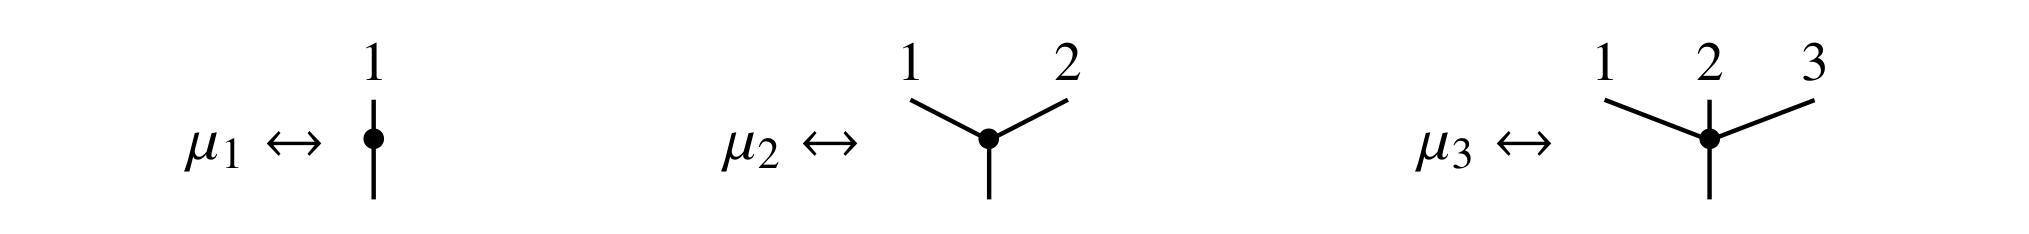
\includegraphics[width=0.95\linewidth]{figures/inline/eq-p42-a.png}% [说明: 该式为原文矢量树图，按原图无损嵌入]
\end{equation*}

上方的叶子解释为相应运算的输入，下方的根为输出。于是上述关系可以通过把一棵树的根嫁接到另一棵树的叶子上，用这些图表示。$Q$ 既是微分又是乘积的导子这一组关系（也称为第一与第二条 $A_\infty$ 关系）可写成：
\begin{equation*}

\includegraphics[width=0.95\linewidth]{figures/inline/eq-p42-b.png}% [说明: 该式为原文矢量树图，按原图无损嵌入]
\end{equation*}

% ==== 原文 PDF 第 43 页 ====
第三条 $A_\infty$ 关系同样可以用树表示：
\begin{equation*}
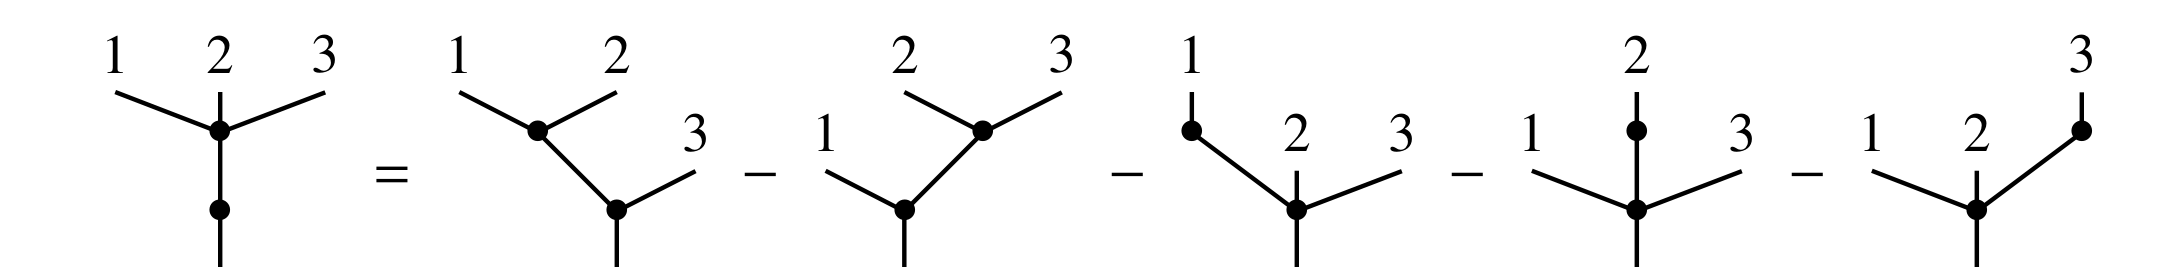
\includegraphics[width=0.95\linewidth]{figures/inline/eq-p43-a.png}% [说明: 该式为原文矢量树图，按原图无损嵌入]
\end{equation*}

可以把这一过程继续到更高的 $n$ 元运算，即更多输入局域算子的情形：对一组 $n$ 个局域算子 $O_1,\ldots,O_n$，存在多种两两碰撞的方式。可以构造一个 $(n-2)$ 维多胞形，称为第 $n$ 个“Sashtev 多胞形”或“结合多面体” $K_n$，其顶点是这些选择，其棱连接由上述某个同伦相联系的两个顶点，其更高维的面则对应这些同伦之复合的同伦，如此类推。
% [原文疑误: 原文正文与 Figure 9 图注均把 Stasheff 多胞形写作 "Sashtev"，应为 "Stasheff"。译文照抄原拼写并保留此注，供作者勘误。]
用 $\mathbb{R}$ 上开区间的构型空间来说，取 $x_1=-x_n$（且 $x_1-x_n>(2n-3)\epsilon$），并考虑
\begin{equation}\tag{3.22}
\mathcal{K}_n(\epsilon) = \{(x_2,\ldots,x_{n-1})\in\mathbb{R}^{n-2} \mid x_i-x_j\ge[2(j-i)-1]\epsilon,\ 1\le i<j\le n\},
\end{equation}
它与 $K_n$ 同胚。上文已看到 $K_2$ 是单点、$K_3$ 是区间。类似地，四个局域算子有五种碰撞方式，可把它们排成五边形 $K_4$ 的顶点；$\mathcal{K}_4(\epsilon)$ 的图示见 Figure 9。
% [Tutor Note: 结合多面体的构型空间实现：条件 $x_i-x_j\ge[2(j-i)-1]\epsilon$ 要求任意两个插入之间隔开足够多的 $\epsilon$；其解集的组合结构正是第 $n$ 个 Stasheff 多胞形，$n=2,3,4$ 分别为点、区间与五边形。]
\begin{figure}[tbp]
  \centering
  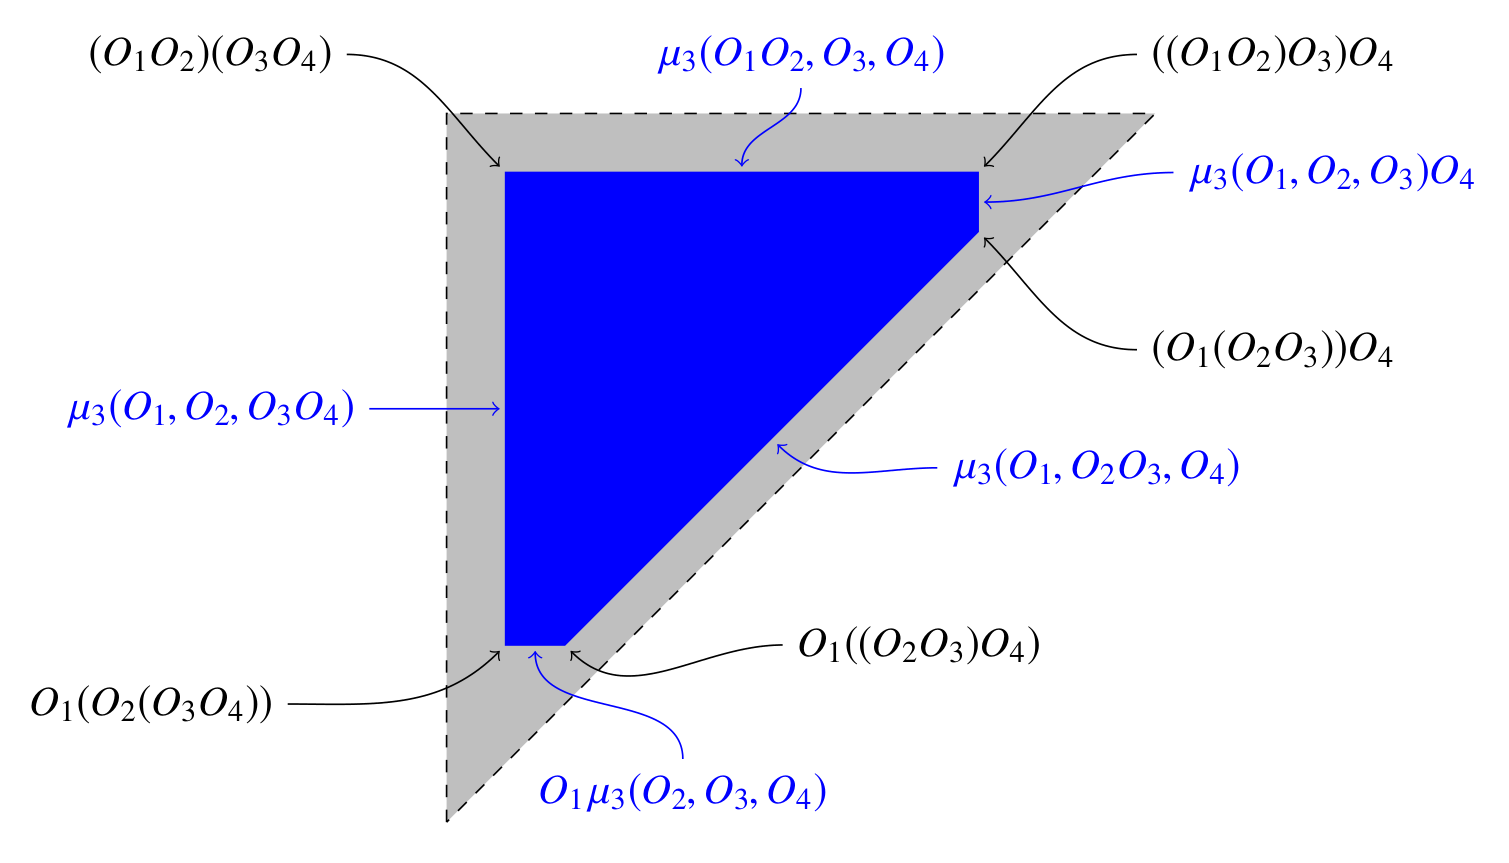
\includegraphics[width=0.80\linewidth]{figures/fig09.png}
  \caption{固定 $x_1$、$x_4$ 时 $\mathbb{R}$ 上 4 个点 $x_1$、$x_2$、$x_3$、$x_4$ 的构型空间。竖直方向对应 $x_2$ 的取值，水平方向对应 $x_3$。第 4 个 Sashtev 多胞形 $K_4$ 与子空间 $\mathcal{K}_4(\epsilon)$ 等同，并以蓝色阴影标出。我们在 $\mathcal{K}_4(\epsilon)$ 的各个角上标出乘积 $O_1O_2O_3O_4$ 中相应的括号配置，并在每条边上标出相应的代数同伦。（原文第 43 页，Figure 9）}
\end{figure}

对每个 $n$，通过拓扑下降构造新的局域算子 $\mu_n(O_1,\ldots,O_n)$（省略插入点 $x_1,\ldots,x_n$）
\begin{equation}\tag{3.23}
\mu_n(O_1,\ldots,O_n) = \lim_{x_1-x_n\to0}\int_{\mathcal{K}_n(\epsilon)}(O_1\cdots O_n)^{(n-2)} = \lim_{x_1-x_n\to0}\int_{\mathcal{K}_n(\epsilon)}O_1O_2^{(1)}\cdots O_{n-1}^{(1)}O_n.
\end{equation}
% ==== 原文 PDF 第 44 页 ====
该运算涉及取 $n-2$ 个后代，因此次数为 $2-n$；即若 $O_i$ 的次数为 $r_i$，则 $\mu_n(O_1,\ldots,O_n)$ 的次数为 $2-n+r_1+\ldots+r_n$。正如 $\mu_3(O_1,O_2,O_3)$ 见证了结合子 $(O_1O_2)O_3 - O_1(O_2O_3)$ 的 $Q$-恰当性，算子 $\mu_n(O_1,\ldots,O_n)$ 也见证了一个更高阶类比物的 $Q$-恰当性：
\begin{equation}\tag{3.24}
\begin{aligned}
Q\mu_n(O_1,\ldots,O_n) &= \sum (-1)^{i+jk+1}(\pm 1)\mu_{i+k+1}\big( O_1,\ldots,O_i,\mu_j(O_{i+1},\ldots,O_{i+j}),O_{i+j+1},\ldots,O_n \big)\\
&\quad + (-1)^n\mu_n(QO_1,\ldots,O_n) + \ldots + (-1)^n(\pm 1)\mu_n(O_1,\ldots,QO_n)\,.
\end{aligned}
\end{equation}
% [存疑: 原文 (3.24) 在句点之后另起一行有一个孤立逗号（疑为排版遗留），译文中从略。]
其中 $(\pm 1)$ 为 Koszul 符号\footnote{Koszul 符号的约定是：对映射 $f:A\to X$ 与 $g:B\to X$（其中 $g$ 为次数 $F(g)$ 的齐次映射），有
\[
(f\otimes g)(a\otimes b) = (-1)^{F(a)F(g)}f(a)\otimes g(b),
\]
其中 $a$ 为次数 $F(a)$ 的齐次元素。这些符号来自：微分 $Q$ 的次数为 1，$\mu_j$ 的次数为 $2-j$。具体地，第一行的 $(\pm 1)$ 是 $(-1)^{F(O_1)+\ldots+F(O_{n-1})}$，第二行的 $(\pm 1)$ 是 $(-1)^{(2-j)(F(O_1)+\ldots+F(O_i))}$。}，求和遍历满足 $i+j+k=n$、$i+k\ge 1$、$j\ge 2$ 的 $i,j,k$。式 (3.24) 称为第 $n$ 条 $A_\infty$ 关系，运算 $\mu_n$ 赋予局域算子 $A_\infty$ 代数的结构。若用一棵有 $n$ 个叶子的有根树表示 $n$ 元运算 $\mu_n$，该关系可图示为：
\begin{equation*}
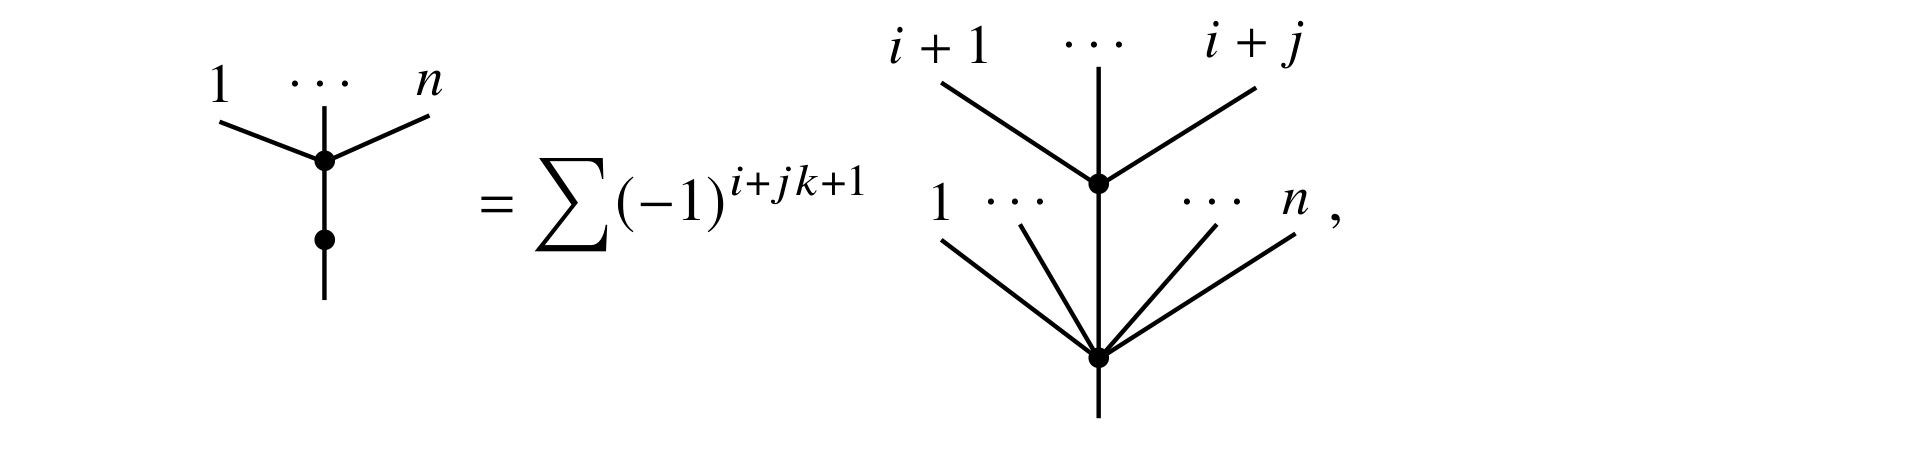
\includegraphics[width=0.95\linewidth]{figures/inline/eq-p44-a.png}% [说明: 该式为原文矢量树图，按原图无损嵌入]
\end{equation*}

这一关系也常直接写成右端那种树的求和，而不加 $i+k\ge 1$ 的限制；我们把 $i=k=0$ 的项分离到左端，以强调它作为某个更高阶结合子的同伦的解释。

可见，$A_\infty$ 代数（有时称为同伦结合代数）是一个（上）链复形 $(A,d_A)$，并带有一族满足上述关系的运算 $\mu_n$。若所有 $\mu_n=0$（$n\ge 3$），则 $A$ 是微分分次结合代数或 DGA：$A$ 是结合代数，并带有微分 $d_A$，它作为结合乘积的导子作用。结果表明，甚至 DGA 的上同调也继承了一个 $A_\infty$ 代数结构，且它与 $(A,d_A)$ 的 $A_\infty$ 结构 $A_\infty$ 等价（参见 [76, Sect. 3.2] 及其中的文献）。

粗略地说，$H^\bullet(A)$ 上的高阶运算度量的是：上同调类所满足的代数关系在它们的链层面提升上失效的程度。同调 $H_\bullet(A)$ 是 $A_\infty$ 代数 $(A,d_A)$ 的极小模型（minimal model）的一例，即其微分为零而高阶运算丰富。
% [背景补充: “极小模型”指与 $A_\infty$ 代数 $(A,d_A)$ 拟同构、但微分取零的结构；它把链层面的同伦信息全部压缩到高阶运算 $\mu_{n\ge 3}$ 中，故 $H^\bullet(A)$ 自然带有 $A_\infty$ 结构。]
另一方面，DGA $(A,d_A)$ 则被称为反极小的，即微分非平凡而高阶运算平凡。$H^\bullet(A)$ 上的这些高阶运算称为 $A_\infty$–Massey 积。它们的优点是极其显式，但依赖于许多选择。数学上称这一过程在拟同构意义下唯一。拟同构就是在上同调上诱导同构的链映射。
% [Tutor Note: 物理图像：$A_\infty$–Massey 积是“上同调类之间的乘积提升到链层面”的障碍；在扭变理论中它们对应只能由 $Q$-闭算子的多点关联函数探测的高阶运算，一般不能由初级乘积重建。]

DGA 的一个简单例子来自通常的 $\mathcal{N}=2$ 超对称量子力学。$\mathcal{N}=2$ 超对称保证存在两个费米子算子 $Q$、$Q^\dagger$，满足 $\{Q^\dagger,Q\}=2H$。我们把该超对称量子力学的算子取作算子代数 $A$，它必然是结合的。设 $A$ 按费米子数算子 $F$ 作 $\mathbb{Z}$-分次，
% [跨页接续: 原文第 44 页/45 页。第 44 页末为 "...Z-graded by the fermion"，第 45 页首为 "number operator F, so that we can write ..."；本分片已把 "fermion number operator F" 一并译出，s03d 应从 "so that we can write $A=\oplus_{j\in\mathbb{Z}}A_j$ ..." 起接续，勿重复 "number operator" 一词。]
